%!TEX root = chapter-methodology.tex
\section{Feature Calculation}
\label{sec:methodology:featurecalc}

Using the ROI obtained from the original 3D palmprint data, three kinds of features to describe the shape of the 3D palmprint: Maximum Depth (MD) of palm center, the Horizontal Cross-section Area (HCA) of different levels and the Radial Line Length (RLL) from the centroid to the boundary of 3D palmprint horizontal cross-section of different levels.

%!TEX root = featurecalc.tex
\subsection{Maximum Depth (MD)}
\label{ssec:methodology:md}

MD means the maximum depth value of the 3D palm from a reference plane. The reference plane is decided using a rectangle obtained by experience. The top left and bottom right pixels of the rectangle are (65,6) and (136,35). These parameters are denoted as $R_s=65, R_e=136, C_s=6$ and $C_e=35$, i.e. the starting(ending) row(column). By examine a random 20 samples, gradient of this area is relatively small.

The depth of the reference plane is defined as the mean depth of the points contained by this rectangle

\begin{equation}
d_r = {1\over{
\sum \limits_{i=R_s}^{R_e} \sum \limits_{j=C_s}^{C_e} m_{ij}
}}
\sum \limits_{i=R_s}^{R_e} \sum \limits_{j=C_s}^{C_e} (d_{ij} \cdot d_{ij})
\end{equation}

where $d_{ij}$ and $m_{ij}$ are the elements defined in ~\ref{eq:methodology:roimatrix} and ~\ref{eq:methodology:roimask}

After getting the depth of the reference plane, we find the maximum depth $d_{max}$ in another region with $R_s=41, R_e=160, C_s=65$ and $C_e=190$.

\begin{equation}
d_{max} = \max \limits_{i=R_s}^{R_e} (\max \limits_{j=C_s}^{C_e} (d_{ij}) )
\end{equation}


The Maximum Depth (MD) is then defined as

\begin{equation}
\label{eq:methodology:md}
MD= d_{max} - d_r
\end{equation}
%!TEX root = featurecalc.tex
\subsection{Horizontal Cross-section Area}
\label{ssec:methodology:hca}

When 3D ROI is examined in a contour view as shown in Figure ~\ref{fig:methodology:roicontour}, it is obvious that the regions of different given depth ranges can be used to describe a sample.

\begin{figure}[htb]
\begin{center}
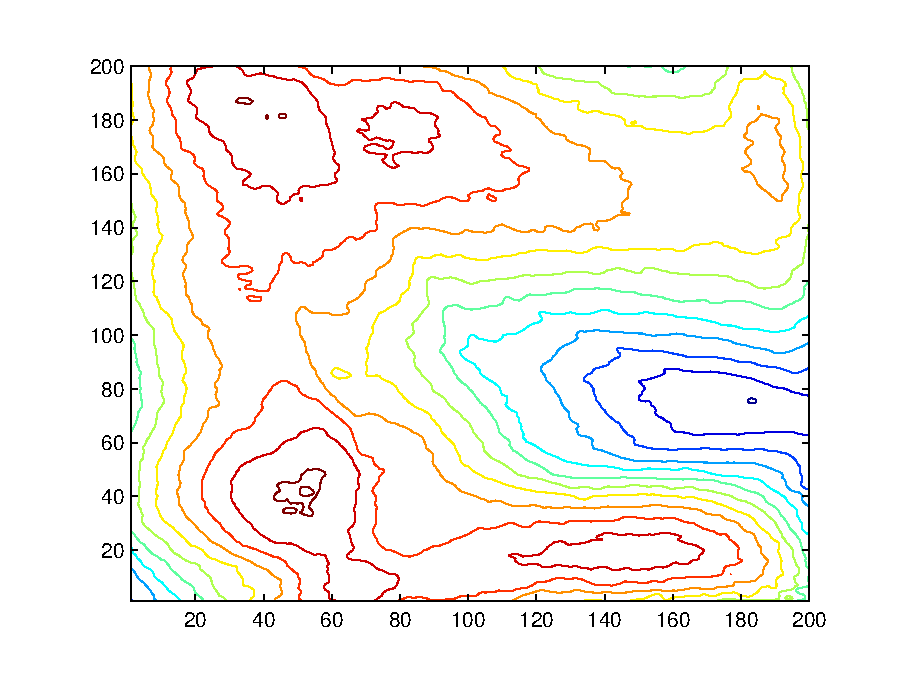
\includegraphics[width=0.9\linewidth]{ch-methodology/figures/roicontour}
\caption[Contour view of a 3D ROI]{Contour view of a 3D ROI}
\label{fig:methodology:roicontour}
\end{center}
\end{figure}

A group of equidistant horizontal planes cut the 3D ROI as shown in Figure ~\ref{fig:methodology:planecut}. Figure ~\ref{fig:methodology:roicontour} shows that most of the deeper level (enclosed with blue curves) are connected. These are more stable in response to noise or transformation.

\begin{figure}[htb]
\begin{center}
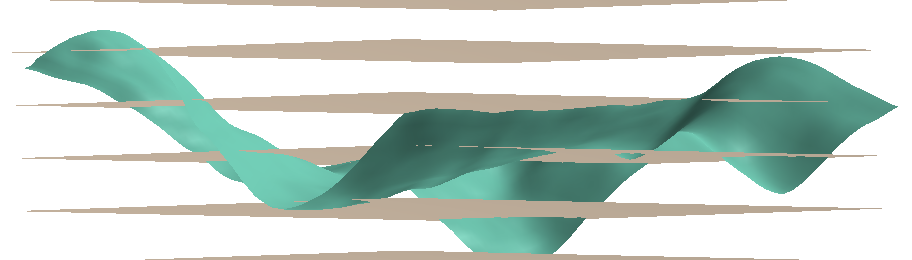
\includegraphics[width=0.9\linewidth]{ch-methodology/figures/planecut}
\caption[3D ROI cut by parallel horizontal planes]{3D ROI cut by parallel horizontal planes}
\label{fig:methodology:planecut}
\end{center}
\end{figure}


To get a stable HCA, we take into consideration only the levels from the deepest point to the reference plane, defined in Section ~\ref{ssec:methodology:md}. Suppose we divide this region into $N$ levels. Every level $G^k, k=1,2,\dots,N$ is described with a 200 by 200 matrix and calculated as

\begin{equation}
G^k_{ij} =
\begin{cases}
1 & \text{if } d_{ij}>h\cdot(N-k+1)/N,\\
0 & \text{otherwise}
\end{cases}
k=1,2,\dots,N;i=1,2,\dots,200;j=1,2,\dots,200;
\end{equation}

where $d_{ij}$ is the depth value of the $i^{th}$ row and $j^{th}$ column pixel of the ROI defined in ~\ref{eq:methodology:roimatrix} and $h$ is the palmprint depth defined by ~\ref{eq:methodology:md}.

To stabilize the areas, the growth of higher level is constrained to its previous level except the first level. That is

\begin{equation}
L^k=
\begin{cases}
G^1                             & k=1 \\
G^k \cap (L^{k-1} \oplus \Theta^{k-1}) & k=2,3,\dots,N
\end{cases}
\end{equation}

where $\cap$ denotes logical AND, $\oplus$ denotes a morphological dilation operation and  $\Theta^{k}$ is a disk morphological structuring element whose size can be calculated by $35-3 \times k$ (which is suitable for N = 8 by experience).

\begin{figure}[htb]
\begin{center}
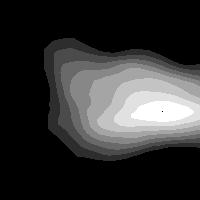
\includegraphics[width=0.9\linewidth]{ch-methodology/figures/hcastack}
\caption[$L^k$ shown stacked when $N=8$]{$L^k$ shown stacked when $N=8$}
\label{fig:methodology:hcastack}
\end{center}
\end{figure}

Figure ~\ref{fig:methodology:hcastack} shows an example of all the levels stacked together.

\begin{figure}[htb]
\centering
\subfigure[$k=1$]{
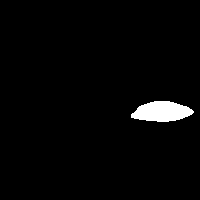
\includegraphics[height=0.18\textheight]{ch-methodology/figures/hca1-1}
\label{fig:methodology:hcalevels:1-1}
}\hspace{0.15\linewidth}
\subfigure[$k=2$]{
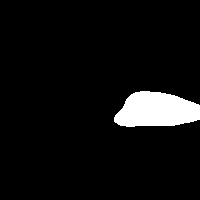
\includegraphics[height=0.18\textheight]{ch-methodology/figures/hca1-2}
\label{fig:methodology:hcalevels:1-2}
}\\
\subfigure[$k=3$]{
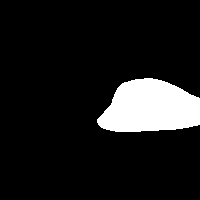
\includegraphics[height=0.18\textheight]{ch-methodology/figures/hca1-3}
\label{fig:methodology:hcalevels:1-3}
}\hspace{0.15\linewidth}
\subfigure[$k=4$]{
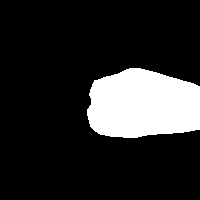
\includegraphics[height=0.18\textheight]{ch-methodology/figures/hca1-4}
\label{fig:methodology:hcalevels:1-4}
}\\
\subfigure[$k=5$]{
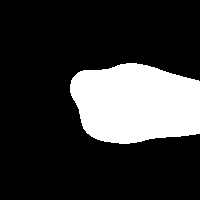
\includegraphics[height=0.18\textheight]{ch-methodology/figures/hca1-5}
\label{fig:methodology:hcalevels:1-5}
}\hspace{0.15\linewidth}
\subfigure[$k=6$]{
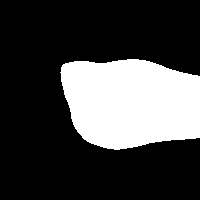
\includegraphics[height=0.18\textheight]{ch-methodology/figures/hca1-6}
\label{fig:methodology:hcalevels:1-6}
}\\
\subfigure[$k=7$]{
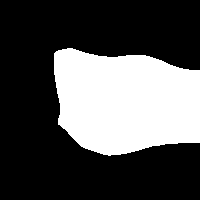
\includegraphics[height=0.18\textheight]{ch-methodology/figures/hca1-7}
\label{fig:methodology:hcalevels:1-7}
}\hspace{0.15\linewidth}
\subfigure[$k=8$]{
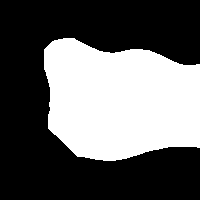
\includegraphics[height=0.18\textheight]{ch-methodology/figures/hca1-8}
\label{fig:methodology:hcalevels:1-8}
}
\caption[$L^k$ of one sample from palm 1]{$L^k$ for $k=1,2,\dots,8$ of a 3D ROI from a palmprint sample}
\label{fig:methodology:hcalevels1}
\end{figure}


\begin{figure}[htb]
\centering
\subfigure[$k=1$]{
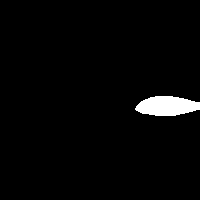
\includegraphics[height=0.18\textheight]{ch-methodology/figures/hca2-1}
}\hspace{0.15\linewidth}
\subfigure[$k=2$]{
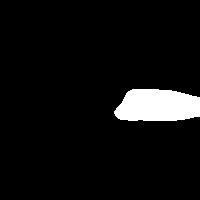
\includegraphics[height=0.18\textheight]{ch-methodology/figures/hca2-2}
}\\
\subfigure[$k=3$]{
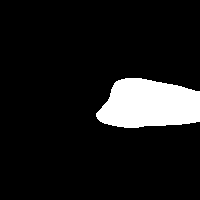
\includegraphics[height=0.18\textheight]{ch-methodology/figures/hca2-3}
}\hspace{0.15\linewidth}
\subfigure[$k=4$]{
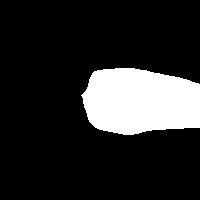
\includegraphics[height=0.18\textheight]{ch-methodology/figures/hca2-4}
}\\
\subfigure[$k=5$]{
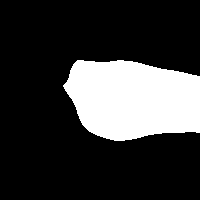
\includegraphics[height=0.18\textheight]{ch-methodology/figures/hca2-5}
}\hspace{0.15\linewidth}
\subfigure[$k=6$]{
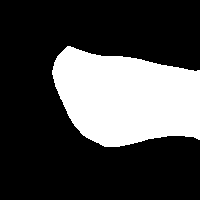
\includegraphics[height=0.18\textheight]{ch-methodology/figures/hca2-6}
}\\
\subfigure[$k=7$]{
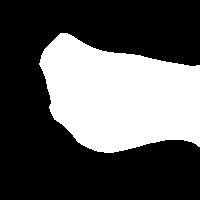
\includegraphics[height=0.18\textheight]{ch-methodology/figures/hca2-7}
}\hspace{0.15\linewidth}
\subfigure[$k=8$]{
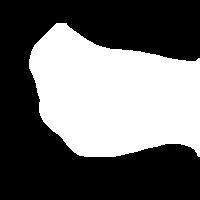
\includegraphics[height=0.18\textheight]{ch-methodology/figures/hca2-8}
}
\caption[$L^k$ of another sample from palm 1]{$L^k$ for $k=1,2,\dots,8$ of a 3D ROI from another palmprint sample from the same person as in Figure ~\ref{fig:methodology:hcalevels1}}
\label{fig:methodology:hcalevels2}
\end{figure}

\begin{figure}[htb]
\centering
\subfigure[$k=1$]{

\includegraphics[height=0.18\textheight]{ch-methodology/figures/hca3-1}
}\hspace{0.15\linewidth}
\subfigure[$k=2$]{

\includegraphics[height=0.18\textheight]{ch-methodology/figures/hca3-2}
}\\
\subfigure[$k=3$]{
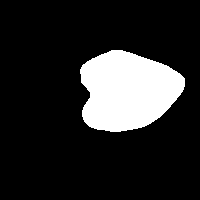
\includegraphics[height=0.18\textheight]{ch-methodology/figures/hca3-3}
}\hspace{0.15\linewidth}
\subfigure[$k=4$]{
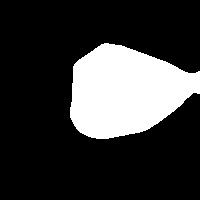
\includegraphics[height=0.18\textheight]{ch-methodology/figures/hca3-4}
}\\
\subfigure[$k=5$]{
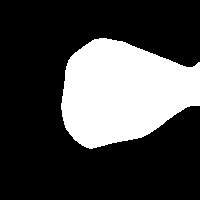
\includegraphics[height=0.18\textheight]{ch-methodology/figures/hca3-5}
}\hspace{0.15\linewidth}
\subfigure[$k=6$]{
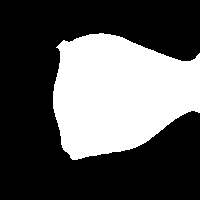
\includegraphics[height=0.18\textheight]{ch-methodology/figures/hca3-6}
}\\
\subfigure[$k=7$]{
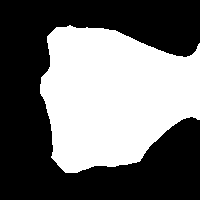
\includegraphics[height=0.18\textheight]{ch-methodology/figures/hca3-7}
}\hspace{0.15\linewidth}
\subfigure[$k=8$]{
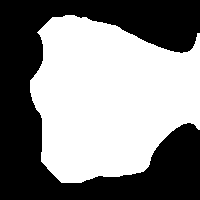
\includegraphics[height=0.18\textheight]{ch-methodology/figures/hca3-8}
}
\caption[$L^k$ of one sample from palm 2]{$L^k$ for $k=1,2,\dots,8$ of a 3D ROI from a palmprint sample from the a different person from that of Figure ~\ref{fig:methodology:hcalevels1}}
\label{fig:methodology:hcalevels3}
\end{figure}

\begin{figure}[htb]
\centering
\subfigure[$k=1$]{

\includegraphics[height=0.18\textheight]{ch-methodology/figures/hca4-1}
}\hspace{0.15\linewidth}
\subfigure[$k=2$]{

\includegraphics[height=0.18\textheight]{ch-methodology/figures/hca4-2}
}\\
\subfigure[$k=3$]{
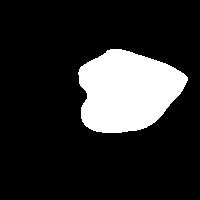
\includegraphics[height=0.18\textheight]{ch-methodology/figures/hca4-3}
}\hspace{0.15\linewidth}
\subfigure[$k=4$]{
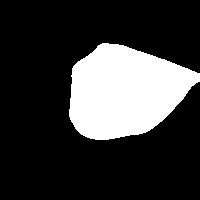
\includegraphics[height=0.18\textheight]{ch-methodology/figures/hca4-4}
}\\
\subfigure[$k=5$]{
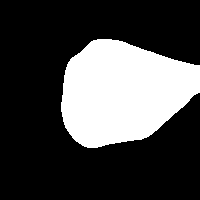
\includegraphics[height=0.18\textheight]{ch-methodology/figures/hca4-5}
}\hspace{0.15\linewidth}
\subfigure[$k=6$]{
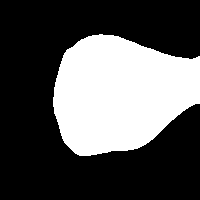
\includegraphics[height=0.18\textheight]{ch-methodology/figures/hca4-6}
}\\
\subfigure[$k=7$]{
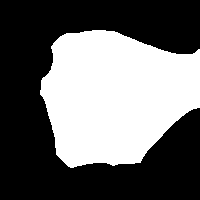
\includegraphics[height=0.18\textheight]{ch-methodology/figures/hca4-7}
}\hspace{0.15\linewidth}
\subfigure[$k=8$]{
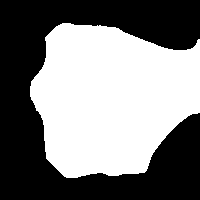
\includegraphics[height=0.18\textheight]{ch-methodology/figures/hca4-8}
}
\caption[$L^k$ of another sample from palm 2]{$L^k$ for $k=1,2,\dots,8$ of a 3D ROI from another palmprint sample from the same person as in Figure ~\ref{fig:methodology:hcalevels3}}
\label{fig:methodology:hcalevels4}
\end{figure}

Figure ~\ref{fig:methodology:hcalevels1} and ~\ref{fig:methodology:hcalevels2} shows the cross-sectional area feature from two samples collected from one palm. Figure ~\ref{fig:methodology:hcalevels3} and ~\ref{fig:methodology:hcalevels4} are extracted from two samples from another palm.

\subsection{Radial Line Length (RLL)}
\label{ssec:methodology:rll}

HCA is a coarse summary of the ROI characteristics. Different sample may have a similar area but dramatically different shape or contour of that area. To describe this shape characteristic, we need more elements to represent the ROI. The Radial Line Length (RLL) is then introduced for this purpose.

First, we calculate the centroid of the first level  $L^1$, thereafter we treat it as the reference point $P_{ref}$ for all levels. Then, from $P_{ref}$ we draw M radial lines which intersect with the contour of every level. RLL is defined as the distance from the intersection point to $P_{ref}$. The radial lines are distributed at equal angles. We record these radial lines from the inner layers to the outer layers starting with the horizontal direction by an $M$ by $N$ dimensional vector
\begin{equation}
R_i, i=1,2,\dots,M\times N
\end{equation}
where $M$ is the number of radial lines and $N$ is the number of cross-sections.

Figure ~\ref{fig:methodology:rll8} through ~\ref{fig:methodology:rll64} show some examples of RLL. This is a more detailed description than HCA as it takes the shape of each area into consideration.

\begin{figure}[htb]
  \begin{center}
    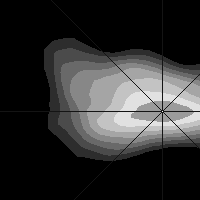
\includegraphics[width=0.4\linewidth]{ch-methodology/figures/rll8}
    \caption[8 radial lines starting from the reference point]{8 radial lines starting from the reference point}
    \label{fig:methodology:rll8}
  \end{center}
\end{figure}

\begin{figure}[htb]
  \begin{center}
    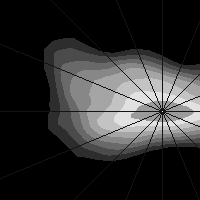
\includegraphics[width=0.4\linewidth]{ch-methodology/figures/rll16}
    \caption[16 radial lines starting from the reference point]{16 radial lines starting from the reference point}
    \label{fig:methodology:rll16}
  \end{center}
\end{figure}

\begin{figure}[htb]
  \begin{center}
    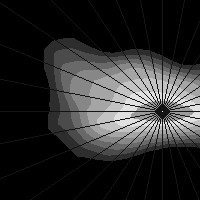
\includegraphics[width=0.4\linewidth]{ch-methodology/figures/rll32}
    \caption[32 radial lines starting from the reference point]{32 radial lines starting from the reference point}
    \label{fig:methodology:rll32}
  \end{center}
\end{figure}

\begin{figure}[htb]
  \begin{center}
    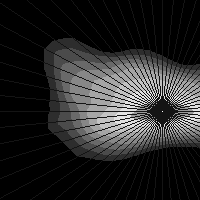
\includegraphics[width=0.4\linewidth]{ch-methodology/figures/rll64}
    \caption[64 radial lines starting from the reference point]{64 radial lines starting from the reference point}
    \label{fig:methodology:rll64}
  \end{center}
\end{figure}



The above three features are mainly determined by the central region of the palm. This region is certainly contained by the ROI described in Section ~\ref{sec:methodology:roiextraction} which makes these features insensitive to translation and rotation. Although the RLL feature can be affected by rotation as the contours change smoothly, if the rotation is small then the variation of the RLL feature will also be small. Actually, there are some restricting pegs on the capture device which can guide the users to put their hands on the proper place as described in ~\cite{Zhang:2009dp}. Furthermore, we assume the user is cooperative when collecting data as we aim at civil rather than law enforcement applications.
